\section{Results}
\label{sec:results}

\subsection{Meta-transcriptomic Recovery Across Spaceflight Accessions}
Mining non-host reads from the six selected OSDR spaceflight datasets revealed that despite pre-flight seed surface sanitation protocols, detectable microbial transcripts were recovered in all whole-seedling accessions (Figure~\ref{fig:study_selection} and Table~\ref{tab:datasets}). Total read depth and the proportion of non-plant reads varied substantially depending on experimental hardware, preservation chemistry, and anatomical tissue type. Whole-seedling experiments preserved in RNAlater or flash-frozen in liquid nitrogen yielded between 0.05\% and 1.8\% non-host reads, corresponding to tens of thousands to hundreds of thousands of high-confidence microbial marker reads per library.

\begin{figure*}[t]
\centering
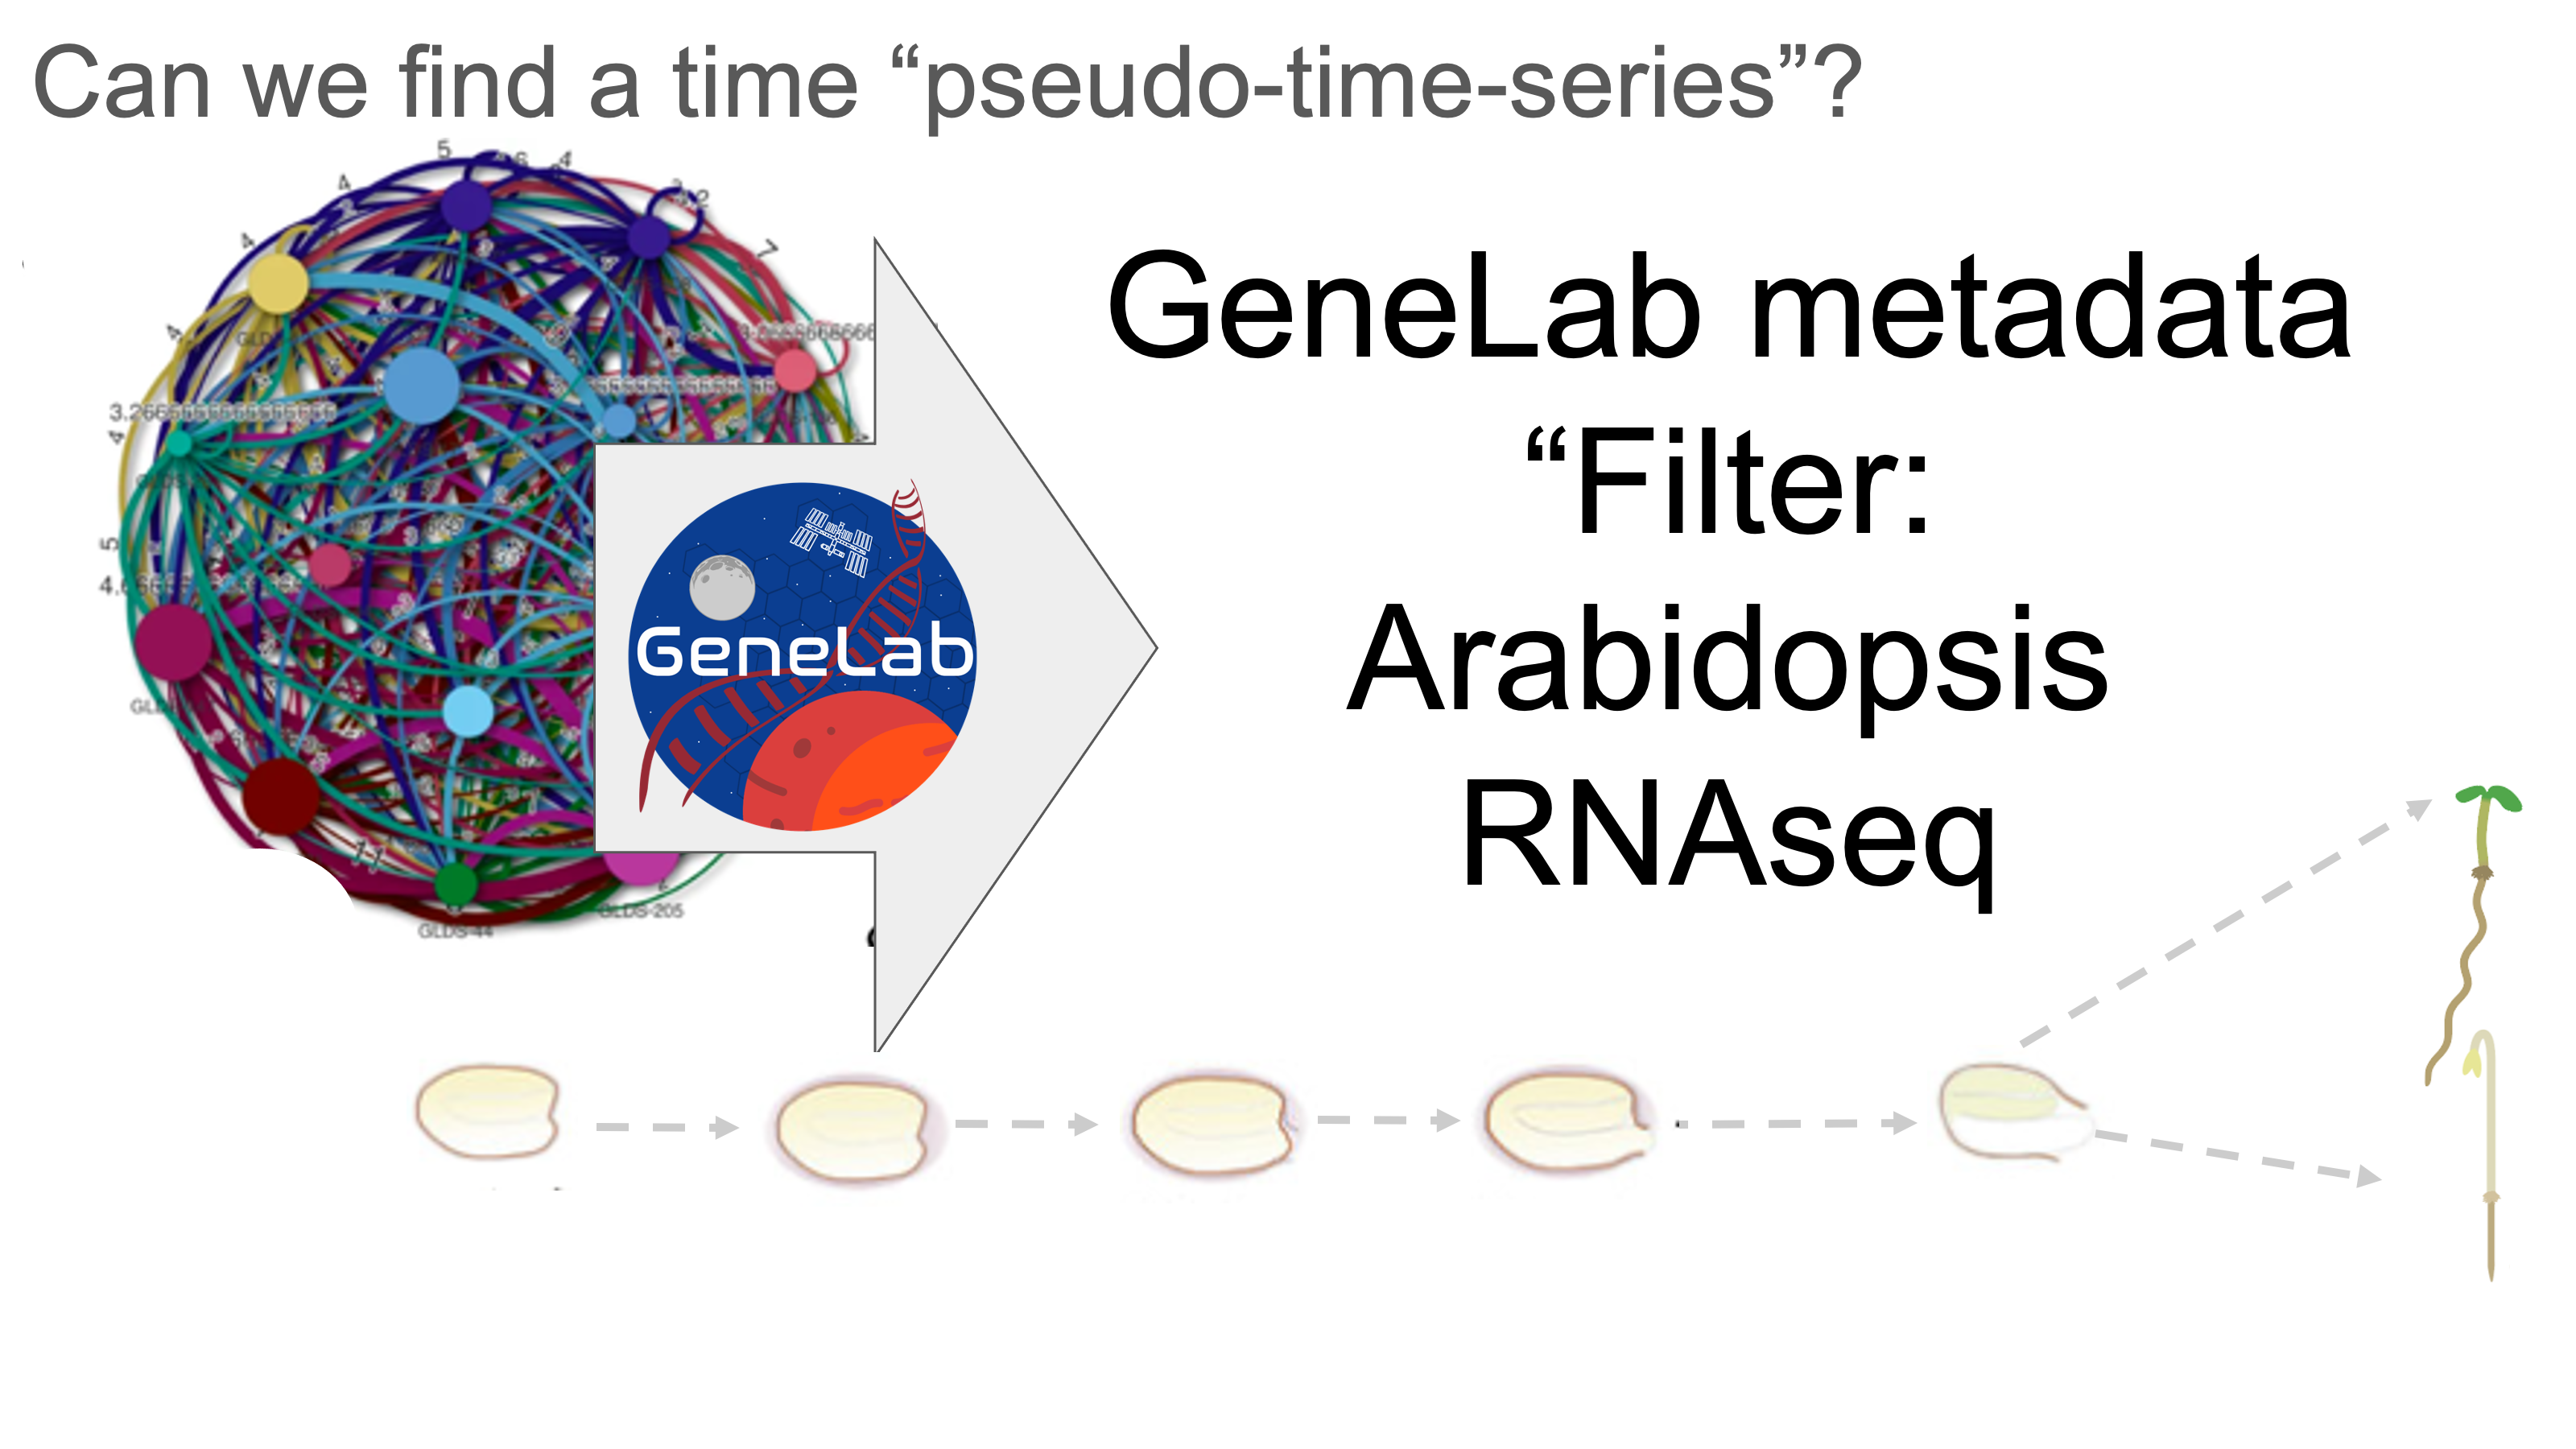
\includegraphics[width=0.85\textwidth]{figures/figure1_study_selection.png}
\caption{\textbf{Systematic selection and environmental parameterization of \textit{Arabidopsis} seedling spaceflight accessions.} Meta-analysis filtering strategy across NASA OSDR repository identifying datasets with overlapping biological replicates, dark/light regimes, and hardware enclosures (BRIC, APEX, EMCS) as described by \citet{barker2023meta}.}
\label{fig:study_selection}
\end{figure*}

\subsection{Pervasive Dominance of \textit{Ralstonia pickettii} in BRIC-19 (OSD-37)}
Taxonomic profiling of 8-day-old etiolated seedlings from the BRIC-19 mission (OSD-37) revealed a consistent microbial consortium across both spaceflight (FL) and ground control (GC) samples (Table~\ref{tab:taxa}). Strikingly, the betaproteobacterium \textit{Ralstonia pickettii} emerged as the overwhelmingly dominant taxon across all biological replicates and ecotypes. In the Cape Verde Islands (Cvi-0) accession, \textit{R. pickettii} accounted for 100\% of all classified microbial reads in multiple samples. In Columbia-0 (Col-0), Wassilewskija-2 (WS-2), and Landsberg \textit{erecta}-0 (Ler-0), \textit{R. pickettii} consistently constituted $>65\%$ of relative abundance.

Beyond \textit{R. pickettii}, OSD-37 libraries contained secondary populations of recognized plant-associated endophytes, including \textit{Herbaspirillum huttiense}, \textit{Pseudomonas fluorescens}, \textit{Curvibacter gracilis}, \textit{Acidovorax temperans}, and \textit{Agrobacterium tumefaciens}. While the primary community composition was conserved between orbit and ground, flight samples exhibited reproducible shifts in the relative abundance of secondary Proteobacteria, suggesting subtle microgravity-mediated or enclosure-induced alterations in host colonization.

\begin{figure*}[t]
\centering
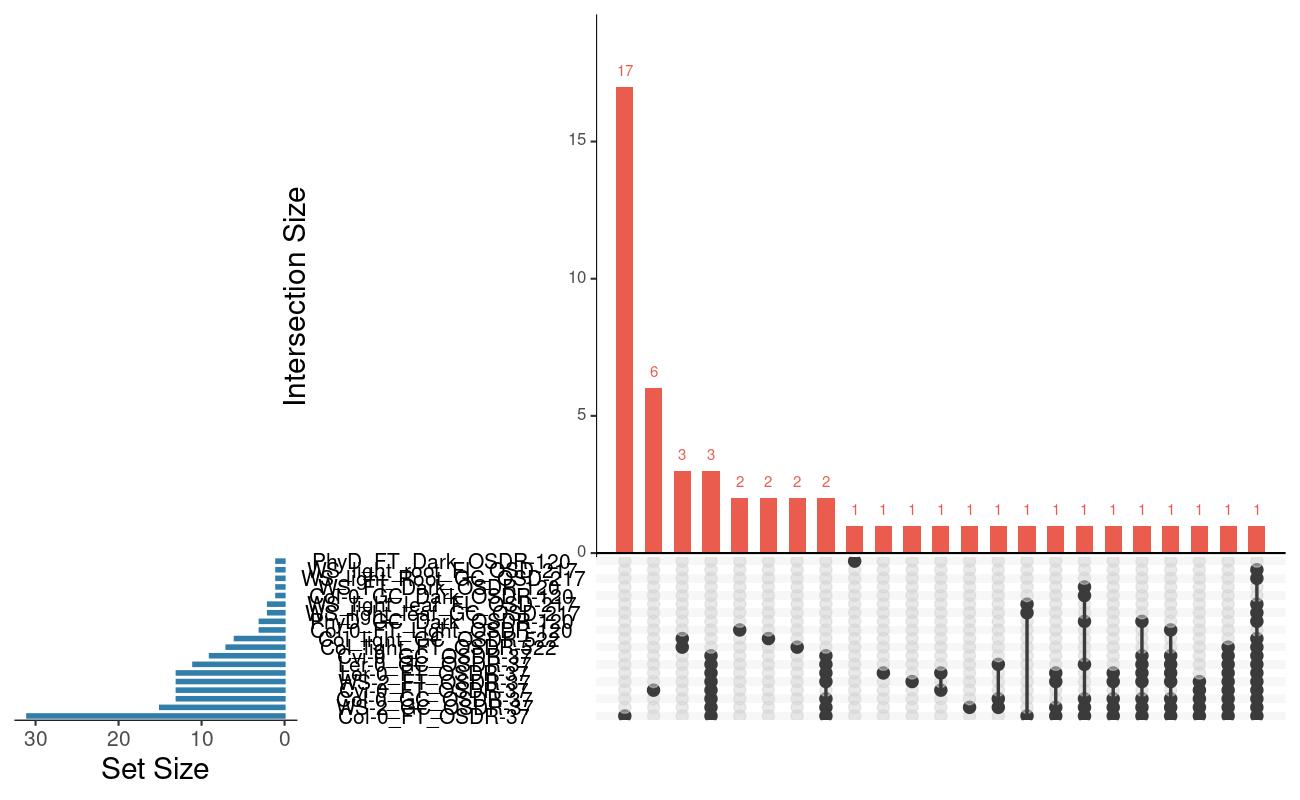
\includegraphics[width=0.92\textwidth]{figures/figure2_upset_plot.png}
\caption{\textbf{UpSet intersection of detected microbial taxa across spaceflight and ground seedling conditions.} Intersections demonstrate a shared core of seed-borne Proteobacteria (including \textit{Ralstonia pickettii} and \textit{Pseudomonas fluorescens}) alongside sample-specific environmental transfers and ecotype-restricted colonizers.}
\label{fig:upset}
\end{figure*}

\subsection{Discovery of \textit{Weizmannia ginsengihumi} in BRIC-20 (OSD-38)}
Analysis of younger 3--4-day-old Col-0 seedlings from BRIC-20 (OSD-38) uncovered a distinctly different microbial profile from the 8-day-old BRIC-19 seedlings. In the Ames Research Center ground control samples preserved via liquid nitrogen fixation (\path{GLDS-38_rna_seq_Atha_WT-Col-0_sl_LN2_Rep1_n2-1}), we identified the firmicute \textit{Weizmannia ginsengihumi} (formerly classified as \textit{Bacillus ginsengihumi}). 

This bacterium, renowned for producing active antioxidants and promoting growth in \textit{Panax ginseng}, had never previously been documented within spaceflight plant tissues or orbital cultivation hardware. Its detection in early germination stages suggests that \textit{W. ginsengihumi} exists as a quiescent seed endophyte that activates upon hydration and imbibition, potentially conferring oxidative stress resilience to the emerging seedling radicle.

\begin{figure*}[t]
\centering
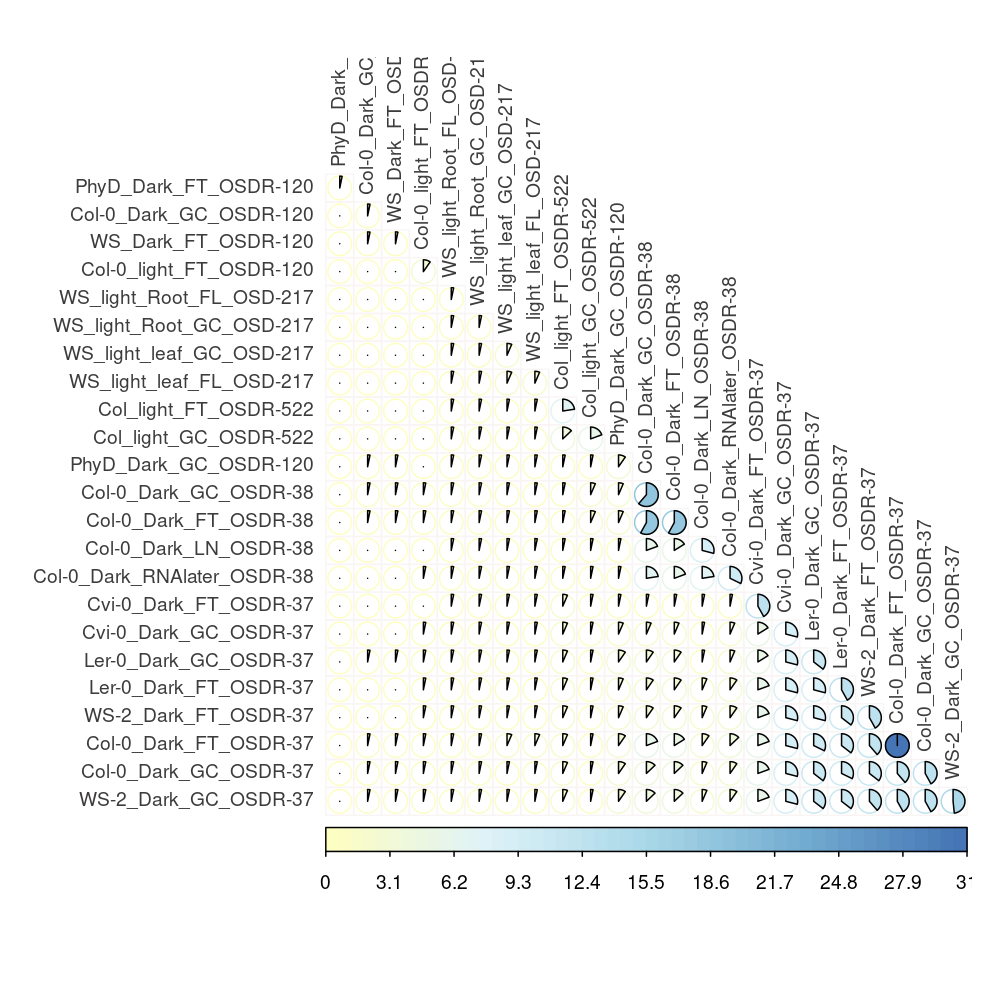
\includegraphics[width=0.88\textwidth]{figures/figure3_correlation_heatmap.png}
\caption{\textbf{Pairwise correlation heatmap of microbial community profiles.} Spearman correlation and hierarchical clustering of microbial profiles across experimental accessions, revealing clustering by mission hardware and plant developmental stage rather than flight status alone.}
\label{fig:heatmap}
\end{figure*}

\subsection{Tissue Partitioning and Microbial Depletion in Root Tips (OSD-120)}
A pivotal question in plant microbiome dynamics is whether endophytes universally colonize all vegetative organs or localize to specific anatomical zones. Analysis of APEX-03-2 (OSD-120), in which 11--13-day-old Col-0 and WS seedlings were grown under directional light regimes and micro-dissected specifically for root tips (apical meristem and elongation zones), produced a dramatic negative result: MetaPhlAn4 profiling reported an absence of detectable microbial taxa across both flight and ground replicates (\path{GLDS-120_rna_seq_Atha_Col-0_root_GC_dark_Rep3} and \path{WS_root_GC_dark_Rep3}).

This finding contrasts sharply with the whole-seedling data from OSD-37, OSD-38, and OSD-522, and with the separated leaf and root tissues of OSD-217. In OSD-217, leaf mesophyll and mature root vasculature harbored robust populations of \textit{Cutibacterium acnes}, \textit{Bradyrhizobium viridifuturi}, and \textit{Delftia acidovorans}. The stark absence of reads in OSD-120 confirms that the active root apical meristem is maintained in a nearly sterile state, while endophytic and epiphytic colonization is compartmentalized in differentiated hypocotyls, cotyledons, and mature vascular bundles.

\begin{figure}[t]
\centering
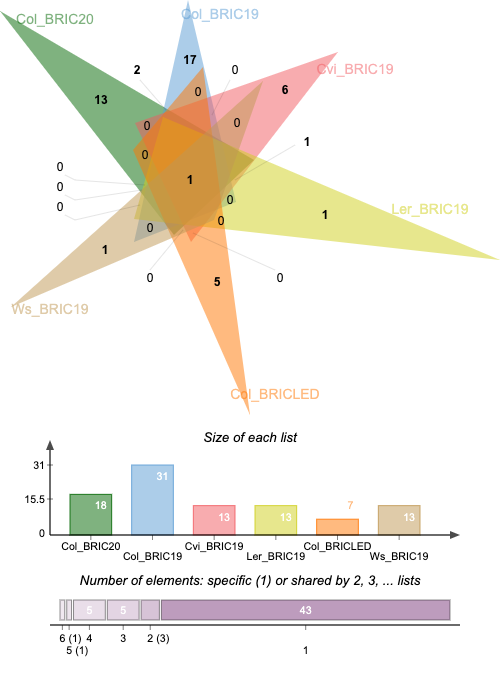
\includegraphics[width=0.48\textwidth]{figures/figure4_venn_chart.png}
\caption{\textbf{jVenn distribution of core seedling microbial associates.} Overlap between major flight experimental cohorts illustrating core persisting taxa versus transient mission-specific contaminants.}
\label{fig:venn}
\end{figure}

\subsection{Partitioning Intrinsic Endophytes from Human and Hardware Commensals}
By cross-referencing all detected taxa against The Microbe Directory and BacDive databases, we categorized the spaceflight seedling metatranscriptome into two distinct ecological guilds (Table~\ref{tab:taxa}):
\begin{enumerate}
    \item \textbf{Seed-Borne Plant Endophytes:} Dominated by environmental Proteobacteria and Firmicutes (\textit{Ralstonia pickettii}, \textit{Pseudomonas fluorescens}, \textit{Herbaspirillum huttiense}, \textit{Agrobacterium tumefaciens}, \textit{Weizmannia ginsengihumi}, \textit{Acidovorax temperans}, and \textit{Paenibacillus} spp.). These taxa were conserved across multiple independent laboratories and mission years, reflecting true internal seed transmission.
    \item \textbf{Human and Hardware Commensals:} Represented by classic human skin and mucosal colonizers, notably \textit{Cutibacterium acnes} (formerly \textit{Propionibacterium acnes}), \textit{Malassezia restricta} (an anthropophilic skin fungus), \textit{Corynebacterium aurimucosum}, \textit{Staphylococcus epidermidis}, and \textit{Escherichia coli}.
\end{enumerate}

These anthropophilic species were recovered consistently from flight hardware (BRIC canisters and Petri plate surfaces), providing direct molecular evidence of payload touch-transfer during pre-flight seed mounting, dish integration, or post-flight harvest on the ISS.
